\section{Database Schema Overview}
\paragraph{}The database schema is structured to support a cryptocurrency wallet application with capabilities for tracking transactions, managing multiple currencies, monitoring exchange rates, and providing user account management. The design employs a robust entity-relationship model with appropriate constraints and data types specific to blockchain data requirements.

The database is organized around five primary entities:

\begin{enumerate}
    \item \textbf{Currency} - Represents different cryptocurrencies or tokens
    \item \textbf{ExchangeRate} - Tracks conversion rates between currencies
    \item \textbf{Transaction} - Records blockchain transactions with detailed metadata
    \item \textbf{User} - Manages application users and authentication
    \item \textbf{Wallet} - Represents cryptocurrency wallets owned by users
\end{enumerate}

Each entity inherits from a common BaseObject type, ensuring consistent handling of identifiers and providing a foundation for entity relationships.
\newpage
\begin{figure}[H]
    \centering
    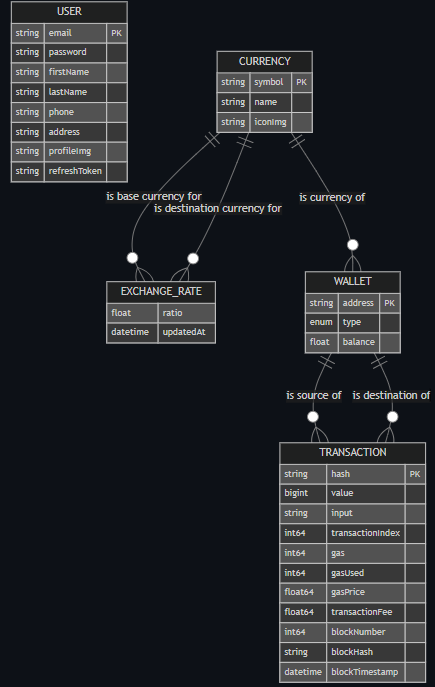
\includegraphics[width= 1\textwidth]{figures/ERD diagram.png}
     \caption{ERD of Database}
    \label{fig:ERD}
\end{figure}
\section{Crypto Exchange Platform Data Models}
% User Model Table
\begin{table}[htbp]
  \centering
  \caption{User}
  \footnotesize
  \renewcommand{\arraystretch}{1.4}
  \setlength{\tabcolsep}{6pt}
  \begin{tabular}{|l|l|c|p{4cm}|p{2.8cm}|}
    \hline
    \textbf{Field} & \textbf{Type} & \textbf{Required} & \textbf{Description} & \textbf{Constraints} \\
    \hline
    email & String & Yes & User email address & Unique \\
    \hline
    normalizedEmail & String & No & Normalized version of email & Unique \\
    \hline
    password & String & Yes & Hashed password & \\
    \hline
    firstName & String & No & User's first name & \\
    \hline
    lastName & String & No & User's last name & \\
    \hline
    fullName & String & No & Computed full name & Computed field \\
    \hline
    phone & String & No & User's phone number & \\
    \hline
    address & String & No & User's physical address & \\
    \hline
    profileImg & String & No & URL to profile image & \\
    \hline
    refreshToken & String & No & Token for authentication refresh & \\
    \hline
  \end{tabular}
\end{table}

% Currency Model Table
\begin{table}[htbp]
  \centering
  \caption{Currency}
  \footnotesize
  \renewcommand{\arraystretch}{1.1}
  \setlength{\tabcolsep}{6pt}
  \begin{tabular}{|l|l|c|p{4cm}|p{2.8cm}|}
    \hline
    \textbf{Field} & \textbf{Type} & \textbf{Required} & \textbf{Description} & \textbf{Constraints} \\
    \hline
    symbol & String & Yes & Currency symbol (e.g., ETH) & Unique \\
    \hline
    name & String & Yes & Full name (e.g., Ethereum) & Unique \\
    \hline
    iconImg & String & Yes & URL to currency icon image & \\
    \hline
  \end{tabular}
\end{table}

% ExchangeRate Model Table
\begin{table}[htbp]
  \centering
  \caption{ExchangeRate}
  \footnotesize
  \renewcommand{\arraystretch}{1.1}
  \setlength{\tabcolsep}{6pt}
  \begin{tabular}{|l|l|c|p{4cm}|p{2.8cm}|}
    \hline
    \textbf{Field} & \textbf{Type} & \textbf{Required} & \textbf{Description} & \textbf{Constraints} \\
    \hline
    ratio & Float64 & Yes & Exchange ratio between currencies & \\
    \hline
    baseCurrency & Currency & Yes & Source currency & Foreign Key \\
    \hline
    destinationCurrency & Currency & Yes & Target currency & Foreign Key \\
    \hline
    updatedAt & DateTime & Yes & Last update timestamp & \\
    \hline
  \end{tabular}
\end{table}

% Wallet Model Table
\begin{table}[htbp]
  \centering
  \caption{Wallet}
  \footnotesize
  \renewcommand{\arraystretch}{1.1}
  \setlength{\tabcolsep}{6pt}
  \begin{tabular}{|l|l|c|p{4cm}|p{2.8cm}|}
    \hline
    \textbf{Field} & \textbf{Type} & \textbf{Required} & \textbf{Description} & \textbf{Constraints} \\
    \hline
    address & String & Yes & Wallet address & Unique \\
    \hline
    type & WalletType & Yes & EOA or Contract & Enum \\
    \hline
    balance & Float64 & Yes & Current balance & Default: 0.0 \\
    \hline
    currency & Currency & Yes & Currency of the wallet & Foreign Key \\
    \hline
  \end{tabular}
\end{table}

% Transaction Model Table
\begin{table}[htbp]
  \centering
  \caption{Transaction}
  \footnotesize
  \renewcommand{\arraystretch}{1.1}
  \setlength{\tabcolsep}{6pt}
  \begin{tabular}{|l|l|c|p{4cm}|p{2.8cm}|}
    \hline
    \textbf{Field} & \textbf{Type} & \textbf{Required} & \textbf{Description} & \textbf{Constraints} \\
    \hline
    hash & String & Yes & Transaction hash & Unique \\
    \hline
    value & BigInt & Yes & Transaction amount & \\
    \hline
    sourceWallet & Wallet & Yes & Source wallet & Foreign Key \\
    \hline
    destinationWallet & Wallet & Yes & Destination wallet & Foreign Key \\
    \hline
    input & String & Yes & Transaction input data & \\
    \hline
    transactionIndex & Int64 & Yes & Index in the block & \\
    \hline
    gas & Int64 & Yes & Gas limit & \\
    \hline
    gasUsed & Int64 & Yes & Gas used & \\
    \hline
    gasPrice & Float64 & Yes & Gas price & \\
    \hline
    transactionFee & Float64 & Yes & Total transaction fee & \\
    \hline
    blockNumber & Int64 & Yes & Block number & \\
    \hline
    blockHash & String & Yes & Block hash & \\
    \hline
    blockTimestamp & DateTime & Yes & Block timestamp & \\
    \hline
  \end{tabular}
\end{table}

% Relationships Table
\begin{table}[htbp]
  \centering
  \caption{Relationships}
  \footnotesize
  \renewcommand{\arraystretch}{1.4}
  \setlength{\tabcolsep}{6pt}
  \begin{tabular}{|l|l|p{7cm}|}
    \hline
    \textbf{Relationship} & \textbf{Type} & \textbf{Description} \\
    \hline
    Currency $\rightarrow$ ExchangeRate & One-to-Many & A currency can be the base for many exchange rates \\
    \hline
    Currency $\rightarrow$ ExchangeRate & One-to-Many & A currency can be the destination for many rates \\
    \hline
    Currency $\rightarrow$ Wallet & One-to-Many & A currency can have many wallets \\
    \hline
    Wallet $\rightarrow$ Transaction (source) & One-to-Many & A wallet can be the source of many transactions \\
    \hline
    Wallet $\rightarrow$ Transaction (dest) & One-to-Many & A wallet can be the destination of many transactions \\
    \hline
  \end{tabular}
\end{table}

% Indexes Table
\begin{table}[htbp]
  \centering
  \caption{Indexes}
  \footnotesize
  \renewcommand{\arraystretch}{1.4}
  \setlength{\tabcolsep}{6pt}
  \begin{tabular}{|l|l|l|p{4.8cm}|}
    \hline
    \textbf{Model} & \textbf{Fields} & \textbf{Type} & \textbf{Description} \\
    \hline
    User & email & Unique & Fast lookup by email \\
    \hline
    Currency & symbol & Unique & Fast lookup by currency symbol \\
    \hline
    Currency & name & Unique & Fast lookup by currency name \\
    \hline
    Wallet & address & Unique & Fast lookup by wallet address \\
    \hline
    Transaction & hash & Unique & Fast lookup by transaction hash \\
    \hline
  \end{tabular}
\end{table}

\begin{table}[htbp]
  \centering
  \caption{Constraints and Validations}
  \footnotesize
  \renewcommand{\arraystretch}{1.4}
  \setlength{\tabcolsep}{6pt}
  \begin{tabular}{|l|l|l|p{5cm}|}
    \hline
    \textbf{Model} & \textbf{Field} & \textbf{Validation} & \textbf{Description} \\
    \hline
    User & email & Exclusive & Email must be unique \\
    \hline
    User & normalizedEmail & Exclusive & Normalized email must be unique \\
    \hline
    Currency & symbol & Exclusive & Currency symbol must be unique \\
    \hline
    Currency & name & Exclusive & Currency name must be unique \\
    \hline
    Wallet & address & Exclusive & Wallet address must be unique \\
    \hline
    Wallet & type & Enum & Must be either EOA or Contract \\
    \hline
    Transaction & hash & Exclusive & Transaction hash must be unique \\
    \hline
  \end{tabular}
\end{table}
\subsection{Example Usage}
\begin{tcolorbox}[width=\textwidth, boxrule=0.5pt, colback=gray!5, colframe=gray!50]
\begin{minted}[fontsize=\small, breaklines=true]{javascript}
// Get a user by email
const user = await e.select(e.User, (user) => ({
  filter_single: { email: 'user@example.com' },
}));

// Get all wallets for a specific currency
const ethWallets = await e.select(e.Wallet, (wallet) => ({
  filter: e.op(wallet.currency.symbol, '=', 'ETH'),
}));

// Get exchange rate between two currencies
const ethToBtcRate = await e.select(e.ExchangeRate, (rate) => ({
  filter_single: {
    baseCurrency: { symbol: 'ETH' },
    destinationCurrency: { symbol: 'BTC' },
  },
}));

// Get all transactions from a specific wallet
const transactions = await e.select(e.Transaction, (tx) => ({
  filter: e.op(tx.sourceWallet.address, '=', '0x123...'),
}));
\end{minted}
\end{tcolorbox}
\section*{Notes and Considerations}

\begin{itemize}
  \item The system uses EdgeDB as the primary database
  \item Wallet balances are stored as float64 which may not be ideal for financial calculations - consider using a fixed-point representation or string-based storage for production
  \item Transaction values are stored as bigint to handle large cryptocurrency amounts
  \item The system currently doesn't have explicit user-wallet ownership relationships - consider adding this if needed
  \item Exchange rates should be regularly updated from external sources
\end{itemize}
\section{User and Cryptocurrency Data Models}
\subsection{Overview}
Core data models for user management, cryptocurrency wallets, transactions, and exchange rates in the COS30049 Blockchain-based Cryptocurrency Exchange platform.
\subsection{Data Models}
\begin{table}[htbp]
  \centering
  \caption{User}
  \renewcommand{\arraystretch}{1.5}
  \begin{tabular}{|p{3cm}|p{2cm}|c|p{4cm}|p{4cm}|}
    \hline
    \textbf{Field} & \textbf{Type} & \textbf{Required} & \textbf{Description} & \textbf{Constraints} \\
    \hline
    email & string & Yes & User email address & Primary Key, Unique \\
    \hline
    normalizedEmail & string & No & Normalized email for case-insensitive lookups & Unique \\
    \hline
    password & string & Yes & Hashed password & \\
    \hline
    firstName & string & No & User's first name & \\
    \hline
    lastName & string & No & User's last name & \\
    \hline
    fullName & string & No & Computed full name & Computed from firstName + lastName \\
    \hline
    phone & string & No & User's phone number & \\
    \hline
    address & string & No & User's physical address & \\
    \hline
    profileImg & string & No & URL to user's profile image & \\
    \hline
    refreshToken & string & No & JWT refresh token & \\
    \hline
  \end{tabular}
\end{table}

\begin{table}[htbp]
  \centering
  \caption{Currency}
  \renewcommand{\arraystretch}{1.5}
  \begin{tabular}{|p{3cm}|p{2cm}|c|p{4cm}|p{4cm}|}
    \hline
    \textbf{Field} & \textbf{Type} & \textbf{Required} & \textbf{Description} & \textbf{Constraints} \\
    \hline
    symbol & string & Yes & Currency symbol (e.g., ETH) & Primary Key, Unique \\
    \hline
    name & string & Yes & Full name (e.g., Ethereum) & Unique \\
    \hline
    iconImg & string & Yes & URL to currency icon image & \\
    \hline
  \end{tabular}
\end{table}

\begin{table}[htbp]
  \centering
  \caption{ExchangeRate}
  \renewcommand{\arraystretch}{1.5}
  \begin{tabular}{|p{3cm}|p{2cm}|c|p{4cm}|p{4cm}|}
    \hline
    \textbf{Field} & \textbf{Type} & \textbf{Required} & \textbf{Description} & \textbf{Constraints} \\
    \hline
    ratio & float64 & Yes & Exchange rate ratio & \\
    \hline
    baseCurrency & Currency & Yes & Reference to base currency & Foreign Key \\
    \hline
    destinationCurrency & Currency & Yes & Reference to destination currency & Foreign Key \\
    \hline
    updatedAt & datetime & Yes & Last update timestamp & \\
    \hline
  \end{tabular}
\end{table}

\begin{table}[htbp]
  \centering
  \caption{Wallet}
  \renewcommand{\arraystretch}{1.5}
  \begin{tabular}{|p{3cm}|p{2cm}|c|p{4cm}|p{4cm}|}
    \hline
    \textbf{Field} & \textbf{Type} & \textbf{Required} & \textbf{Description} & \textbf{Constraints} \\
    \hline
    address & string & Yes & Wallet address & Primary Key, Unique \\
    \hline
    type & enum & Yes & Wallet type (EOA or Contract) & \\
    \hline
    balance & float64 & Yes & Current balance & Default: 0.0 \\
    \hline
    currency & Currency & Yes & Reference to currency & Foreign Key \\
    \hline
  \end{tabular}
\end{table}

\begin{table}[htbp]
  \centering
  \caption{Transaction}
  \renewcommand{\arraystretch}{1.5}
  \begin{tabular}{|p{3cm}|p{2cm}|c|p{4cm}|p{4cm}|}
    \hline
    \textbf{Field} & \textbf{Type} & \textbf{Required} & \textbf{Description} & \textbf{Constraints} \\
    \hline
    hash & string & Yes & Transaction hash & Primary Key, Unique \\
    \hline
    value & bigint & Yes & Transaction amount & \\
    \hline
    sourceWallet & Wallet & Yes & Reference to source wallet & Foreign Key \\
    \hline
    destinationWallet & Wallet & Yes & Reference to destination wallet & Foreign Key \\
    \hline
    input & string & Yes & Transaction input data & \\
    \hline
    transactionIndex & int64 & Yes & Index in the block & \\
    \hline
    gas & int64 & Yes & Gas limit & \\
    \hline
    gasUsed & int64 & Yes & Gas used & \\
    \hline
    gasPrice & float64 & Yes & Gas price & \\
    \hline
    transactionFee & float64 & Yes & Total transaction fee & \\
    \hline
    blockNumber & int64 & Yes & Block number & \\
    \hline
    blockHash & string & Yes & Block hash & \\
    \hline
    blockTimestamp & datetime & Yes & Block timestamp & \\
    \hline
  \end{tabular}
\end{table}

\begin{table}[htbp]
  \centering
  \caption{Relationships}
  \renewcommand{\arraystretch}{1.5}
  \begin{tabular}{|p{5.5cm}|p{3cm}|p{6cm}|}
    \hline
    \textbf{Relationship} & \textbf{Type} & \textbf{Description} \\
    \hline
    User$\rightarrow$Wallet & One-to-Many & A user can own multiple wallets \\
    \hline
    Currency$\rightarrow$Wallet & One-to-Many & A currency can be used by multiple wallets \\
    \hline
    Currency$\rightarrow$ExchangeRate (base) & One-to-Many & A currency can be the base in multiple exchange rates \\
    \hline
    Currency$\rightarrow$ExchangeRate (destination) & One-to-Many & A currency can be the destination in multiple exchange rates \\
    \hline
    Wallet$\rightarrow$Transaction (source) & One-to-Many & A wallet can be the source of multiple transactions \\
    \hline
    Wallet$\rightarrow$Transaction (destination) & One-to-Many & A wallet can be the destination of multiple transactions \\
    \hline
  \end{tabular}
\end{table}

\begin{table}[htbp]
  \centering
  \caption{Indexes}
  \renewcommand{\arraystretch}{1.5}
  \begin{tabular}{|p{3cm}|p{3cm}|p{3cm}|p{6cm}|}
    \hline
    \textbf{Model} & \textbf{Fields} & \textbf{Type} & \textbf{Description} \\
    \hline
    User & email & Unique & Fast lookup by email \\
    \hline
    User & normalizedEmail & Unique & Case-insensitive email lookup \\
    \hline
    Currency & symbol & Unique & Fast lookup by symbol \\
    \hline
    Currency & name & Unique & Fast lookup by name \\
    \hline
    Wallet & address & Unique & Fast lookup by wallet address \\
    \hline
    Transaction & hash & Unique & Fast lookup by transaction hash \\
    \hline
  \end{tabular}
\end{table}

\begin{table}[htbp]
  \centering
  \caption{Constraints and Validations}
  \renewcommand{\arraystretch}{1.5}
  \begin{tabular}{|p{3cm}|p{4.5cm}|p{7cm}|}
    \hline
    \textbf{Model} & \textbf{Constraint} & \textbf{Description} \\
    \hline
    User & Email format & Email must be in valid format \\
    \hline
    User & Password complexity & Password must meet complexity requirements \\
    \hline
    Currency & Symbol format & Symbol must be uppercase letters \\
    \hline
    Wallet & Address format & Address must be valid blockchain address \\
    \hline
    Transaction & Positive value & Transaction value must be positive \\
    \hline
    Transaction & Source != Destination & Source and destination wallets must differ \\
    \hline
  \end{tabular}
\end{table}
\subsection{Example Use}
\subsubsection*{Creating a User}
\begin{tcolorbox}[width=\textwidth, boxrule=0.5pt, colback=gray!5, colframe=gray!50]
\begin{minted}[fontsize=\small, breaklines=true]{javascript}
const user = await e.insert(e.User, {
  email: 'user@example.com',
  normalizedEmail: 'user@example.com'.toLowerCase(),
  password: await bcrypt.hash('securePassword123', 10),
  firstName: 'John',
  lastName: 'Doe',
  phone: '+1234567890',
  address: '123 Main St, City, Country',
});
\end{minted}
\end{tcolorbox}
\subsubsection*{Creating a Wallet}
\begin{tcolorbox}[width=\textwidth, boxrule=0.5pt, colback=gray!5, colframe=gray!50]
\begin{minted}[fontsize=\small, breaklines=true]{javascript}
const currency = await e.select(e.Currency, (c) => ({
  filter: e.op(c.symbol, '=', 'ETH'),
}));

const wallet = await e.insert(e.Wallet, {
  address: '0x742d35Cc6634C0532925a3b844Bc454e4438f44e',
  type: 'EOA',
  balance: 1.25,
  currency: currency,
});
\end{minted}
\end{tcolorbox}
\subsubsection*{Querying Transactions}
\begin{tcolorbox}[width=\textwidth, boxrule=0.5pt, colback=gray!5, colframe=gray!50]
\begin{minted}[fontsize=\small, breaklines=true]{javascript}
const transactions = await e.select(e.Transaction, (t) => ({
  filter: e.op(
    t.sourceWallet.address,
    '=',
    '0x742d35Cc6634C0532925a3b844Bc454e4438f44e',
  ),
  order_by: {
    expression: t.blockTimestamp,
    direction: e.DESC,
  },
  limit: 10,
}));
\end{minted}
\end{tcolorbox}
